\chapter{鮮度の表現方法の策定}
\label{chap:verification}

本章では,視覚化システムで採用する鮮度の表現方法を策定する.

実際のブラウザ画面をキャプチャした画像を画像編集ソフトで加工し,システムで採用される候補の表現方法をそれぞれ適用する.

鮮度の視覚化が適用された画像を見て,各表現方法を評価する.

\newpage

評価する全ての表現方法に関して図\ref{fig:ver-base}をベースに加工する.

\begin{figure}[htbp]
  \begin{center}
    \fbox{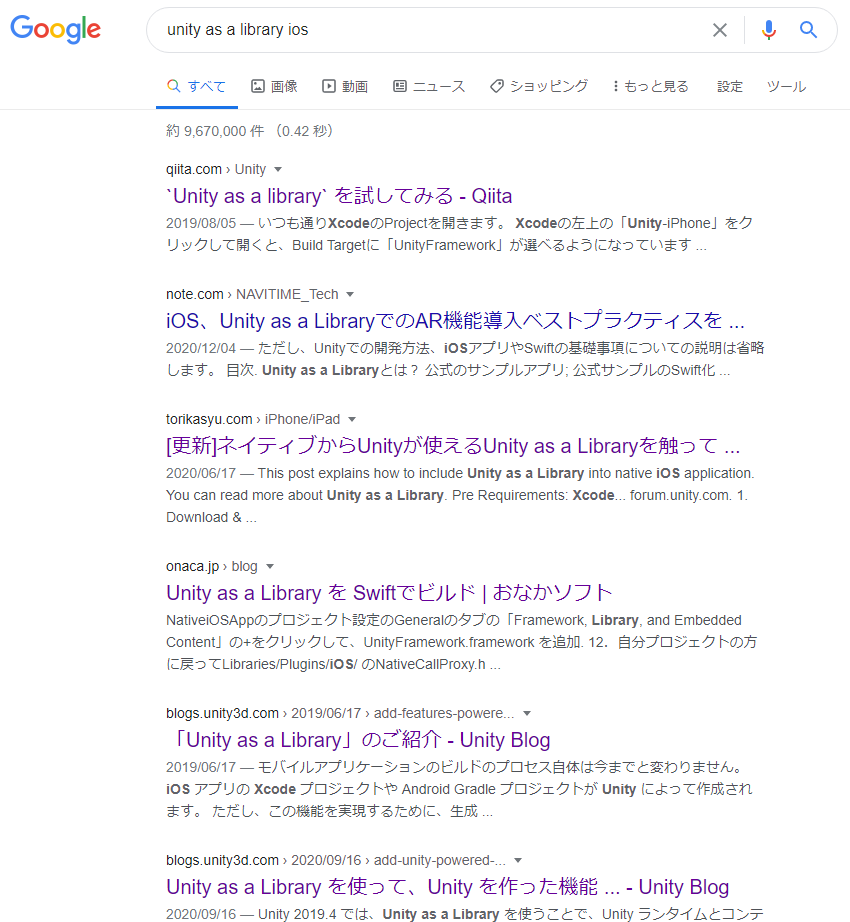
\includegraphics[width=60mm]{images/base.png}}
  \end{center}
  \caption{視覚化前の検索結果一覧画面}
  \label{fig:ver-base}
\end{figure}

各表現方法は類似した系統ごとに,分類して紹介する.

\section{テクスチャによる表現方法}
\label{sec:ver-texture}

\subsection{紙の経年劣化}
\label{subsec:ver-tex-sheet}

紙は時間が経つと黄ばみやシミができる.そういった変化を参考に,情報の鮮度を視覚化した.

\begin{figure}[htbp]
  \begin{minipage}{0.5\hsize}
    \begin{center}
      \fbox{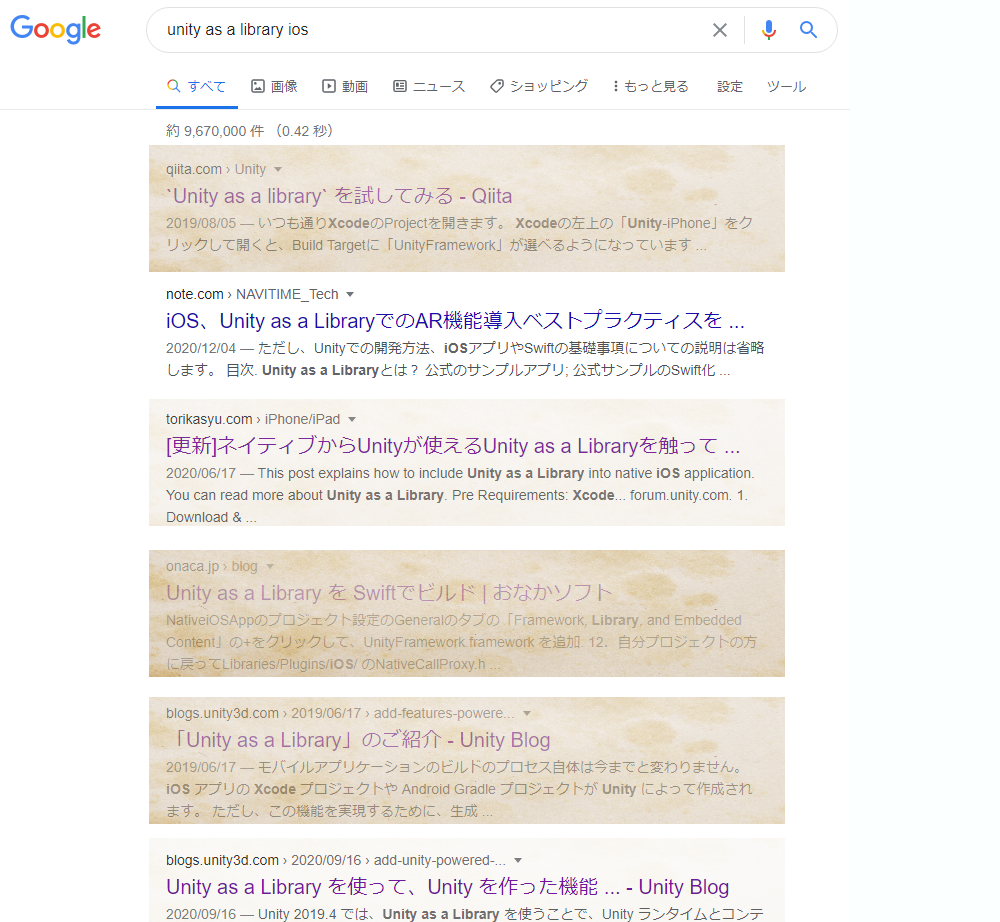
\includegraphics[width=60mm]{images/sheet-degradation1.png}}
    \end{center}
    \caption{紙の経年劣化をイメージした視覚化1}
    \label{fig:ver-sheet1}
  \end{minipage}
  \begin{minipage}{0.5\hsize}
    \begin{center}
      \fbox{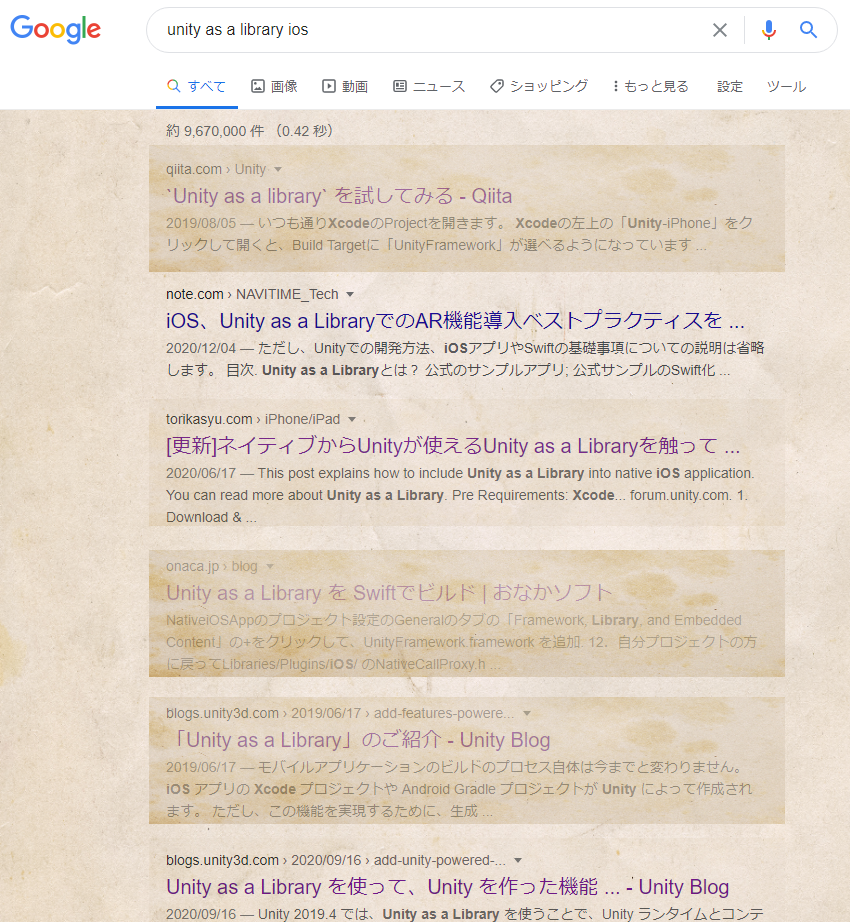
\includegraphics[width=60mm]{images/sheet-degradation2.png}}
    \end{center}
    \caption{紙の経年劣化をイメージした視覚化2}
    \label{fig:ver-sheet2}
  \end{minipage}
\end{figure}

図\ref{fig:ver-sheet1}は,各検索結果ごとの公開日を参考に,劣化した紙のテクスチャを適用している.

図\ref{fig:ver-sheet2}は,劣化した紙のテクスチャが背景になじむように,全体に紙のテクスチャを適用して調整している.

紙の劣化を参考にしているため,各情報の古さが分かりやすい.家や図書館などで古くなった本を見た経験があれば,紙の時間経過による劣化を連想しやすい.

図\ref{fig:ver-sheet1}に比べて,図\ref{fig:ver-sheet2}は背景に紙のテクスチャを設定しているため劣化した紙のテクスチャに違和感が少ない.

\subsection{金属のさび}
\label{subsec:ver-tex-russet}

金属は雨風にさらされてさびが発生するため,時間経過による劣化が簡単に見て取れる.これを参考に視覚化した.

\begin{figure}[htbp]
  \begin{minipage}{0.5\hsize}
    \begin{center}
      \fbox{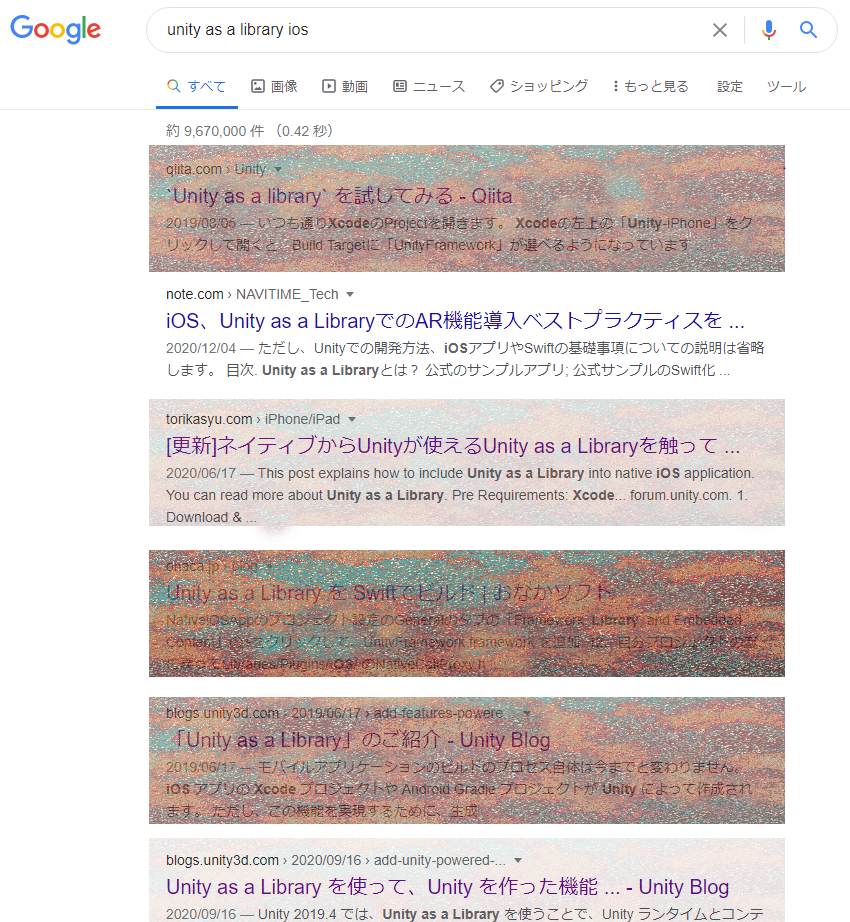
\includegraphics[width=60mm]{images/iron-russet1.png}}
    \end{center}
    \caption{金属のさびをイメージした視覚化1}
    \label{fig:ver-russet1}
  \end{minipage}
  \begin{minipage}{0.5\hsize}
    \begin{center}
      \fbox{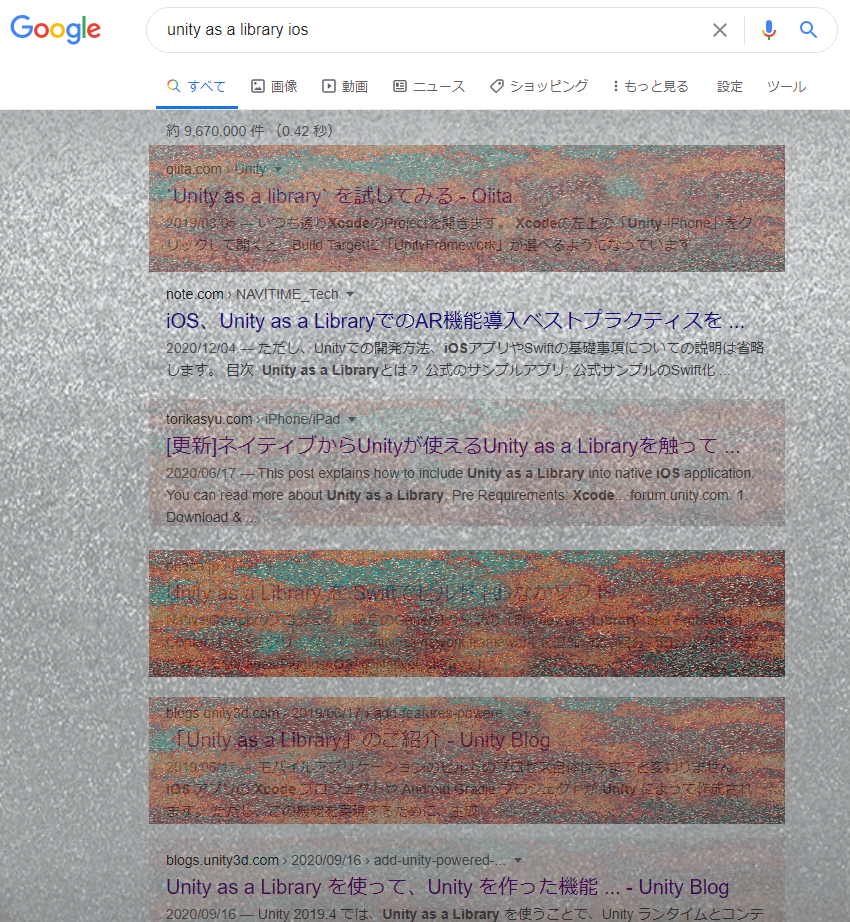
\includegraphics[width=60mm]{images/iron-russet2.png}}
    \end{center}
    \caption{金属のさびをイメージした視覚化2}
    \label{fig:ver-russet2}
  \end{minipage}
\end{figure}

\ref{subsec:ver-tex-sheet}の方法と同様に,図\ref{fig:ver-russet1}は錆びた金属のテクスチャを適用している.

また,図\ref{fig:ver-russet2}は,背景に錆びていない金属のテクスチャを適用している.

\ref{subsec:ver-tex-sheet}と比べて古い情報が強調されているが,背景に金属のテクスチャを適用してもぬぐい切れない不自然さがある.

これは,文字が記録されている媒体として,金属があまり適していないためだと推測する.

\section{色による変化}
\label{sec:ver-color}

\subsection{背景の色褪せ}
\label{subsec:ver-col-cor}

実世界のモノが腐食するイメージを参考に,背景の色褪せによって情報の鮮度を視覚化した.

\begin{figure}[htbp]
  \begin{minipage}{0.5\hsize}
    \begin{center}
      \fbox{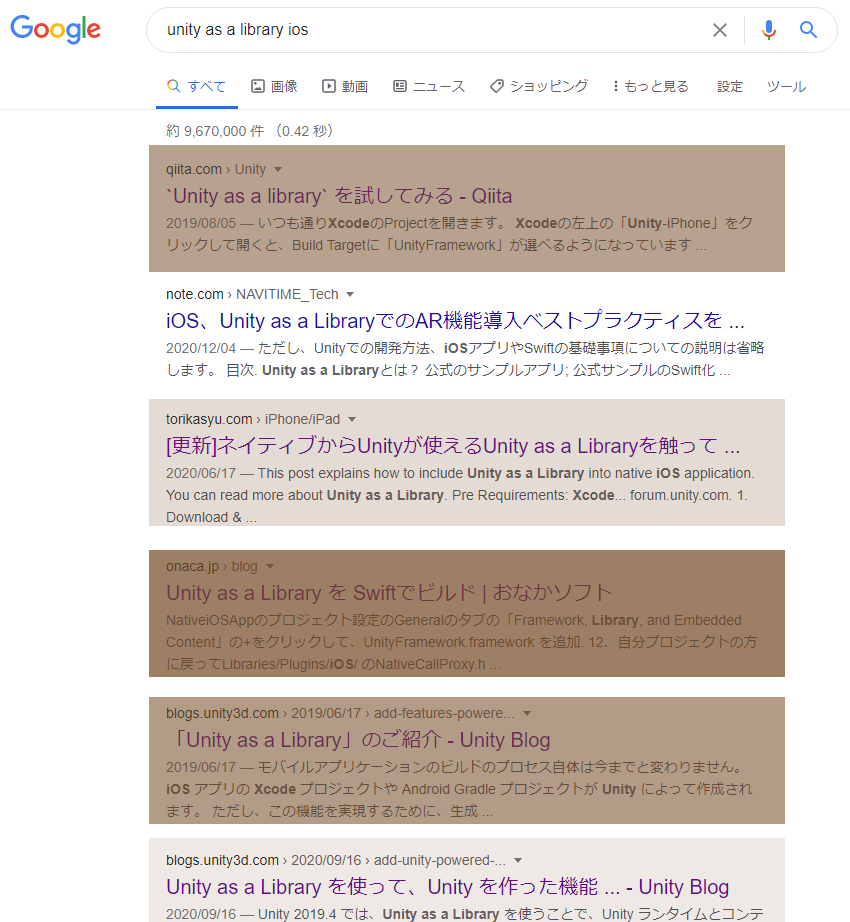
\includegraphics[width=60mm]{images/corrosion1.png}}
    \end{center}
    \caption{腐食をイメージした視覚化1}
    \label{fig:ver-corrosion1}
  \end{minipage}
  \begin{minipage}{0.5\hsize}
    \begin{center}
      \fbox{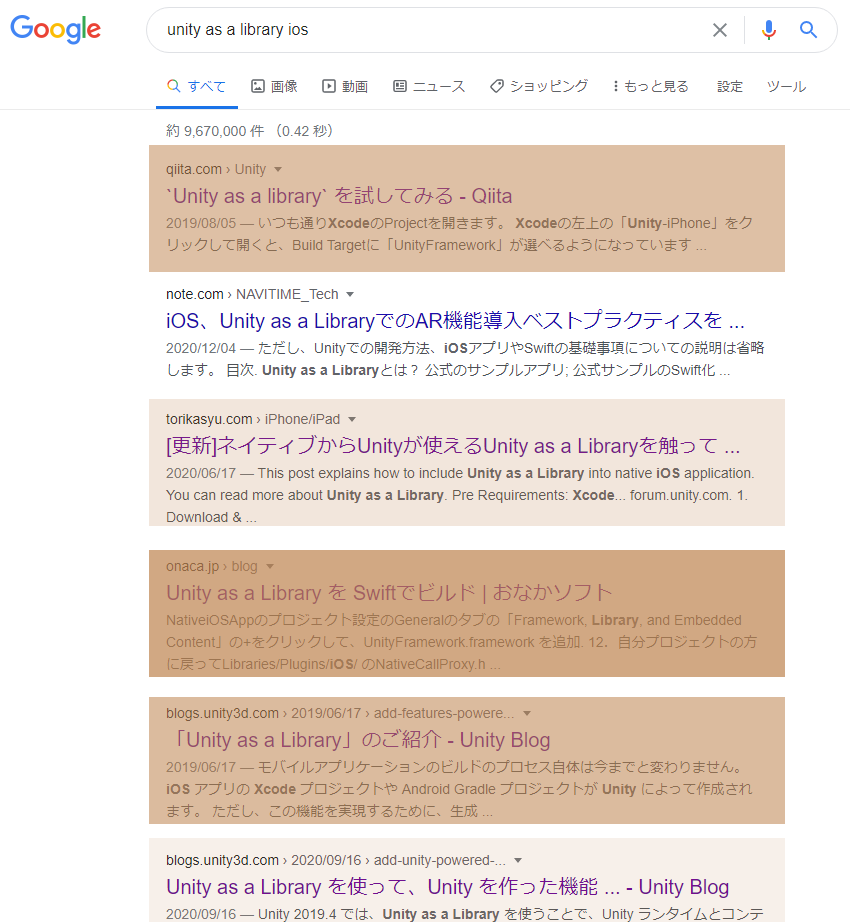
\includegraphics[width=60mm]{images/corrosion2.png}}
    \end{center}
    \caption{腐食をイメージした視覚化2}
    \label{fig:ver-corrosion2}
  \end{minipage}
\end{figure}

図\ref{fig:ver-corrosion1},図\ref{fig:ver-corrosion2}は共に腐食を参考にしたため,暗い茶色や赤茶色の中で,鮮度ごとに色が変化するように視覚化を適用している.

コンセプトとしては\ref{sec:ver-texture}で検証した二つと近いが,こちらの方が外見的にシンプルである.そのため,元の白い背景に対して不自然さが少ないが,色の変化が鮮度を示していることを認識しにくい.

永井\cite{fading}らの実験によれば,黄色方向への色変化やムラを加えることが,古さを感じさせる手法として有効とあるが,検索結果一覧では元が文章であるため変化が乏しい.

適応する色の選定部分において議論の余地がある.

\subsection{インクの劣化}
\label{subsec:ver-col-ink}

紙に書いた文字のインクは時間経過によって劣化していく.そういった変化を参考に,情報の鮮度を視覚化した.

\begin{figure}[htbp]
  \begin{minipage}{0.5\hsize}
    \begin{center}
      \fbox{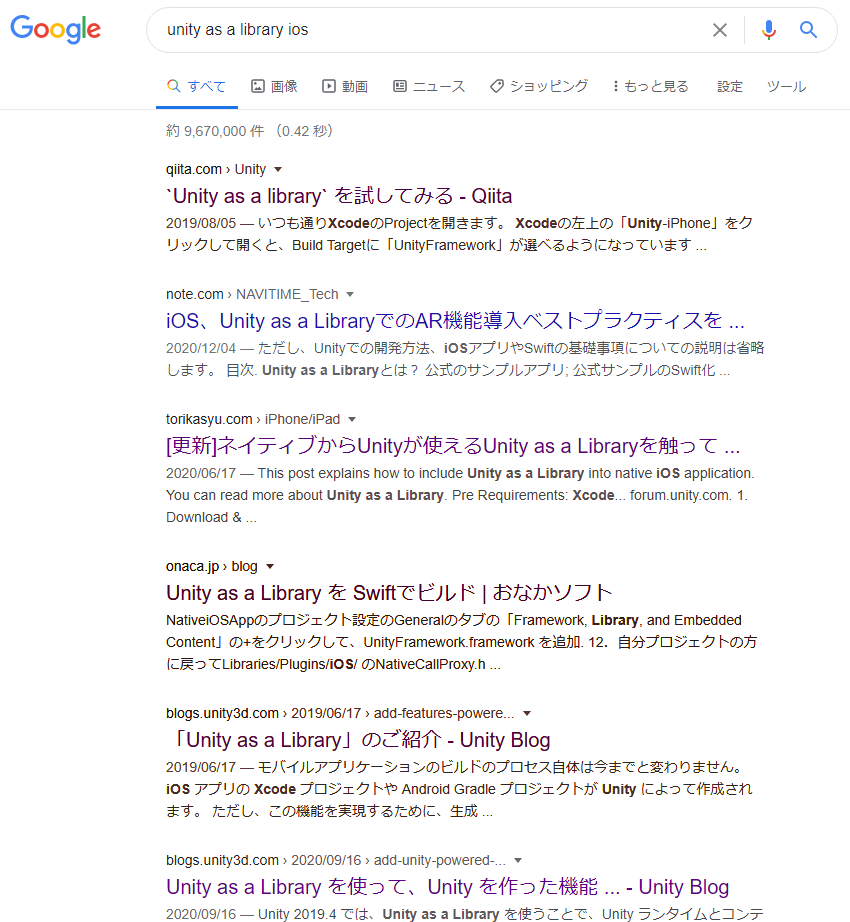
\includegraphics[width=60mm]{images/ink1.png}}
    \end{center}
    \caption{インクの劣化をイメージした視覚化1}
    \label{fig:ver-ink1}
  \end{minipage}
  \begin{minipage}{0.5\hsize}
    \begin{center}
      \fbox{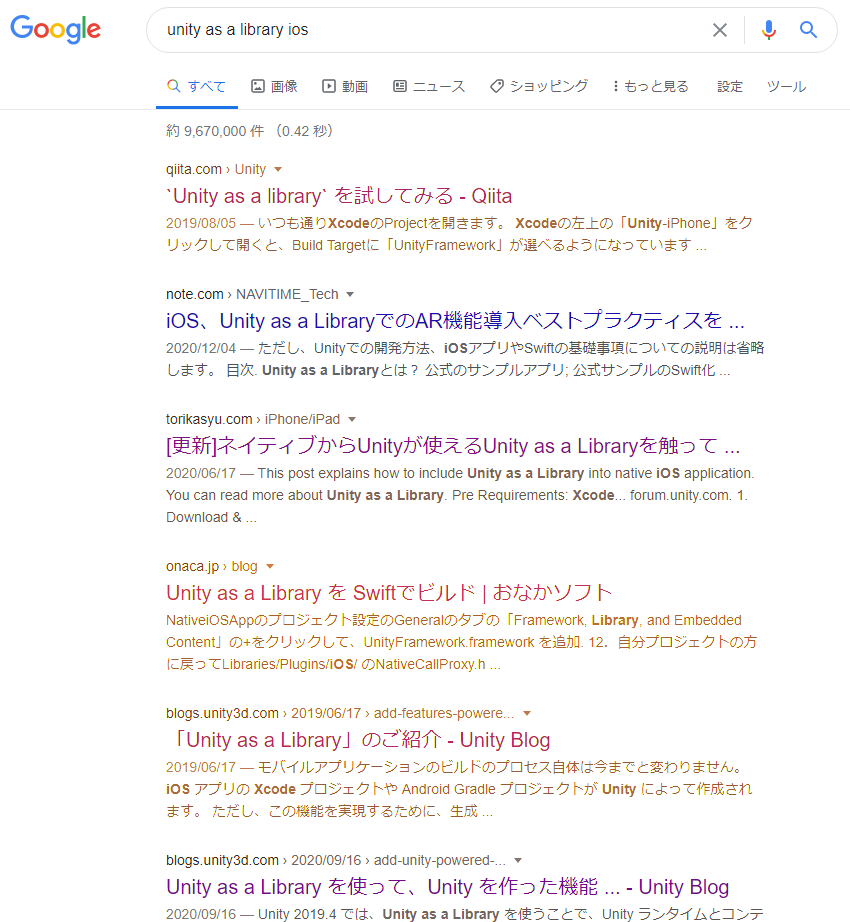
\includegraphics[width=60mm]{images/ink2.png}}
    \end{center}
    \caption{インクの劣化をイメージした視覚化2}
    \label{fig:ver-ink2}
  \end{minipage}
\end{figure}

\ref{subsec:ver-col-cor}と同様に,図\ref{fig:ver-ink1}では,情報の鮮度に応じて文字の色が焦げ茶色に近づいている.

また,図\ref{fig:ver-ink2}は,背景色の白に薄まるように変化を加えている.

図\ref{fig:ver-ink1}は,視覚化による変化が目立たなかった.これではユーザに情報の鮮度を認識させるという目的が果たせていない.

図\ref{fig:ver-ink2}は,古い印象を与えることには成功している.しかし,古いか新しいかの二択に捉えられやすい.

どちらの場合も段階的な変化を認識しやすい視覚化の方法とは言えない.

\section{文字の消失による変化}
\label{sec:ver-character}

\subsection{透明化}
\label{subsec:ver-chr-trp}

実世界のモノは時間経過によって風化していく.その消失していくさまをイメージして,各項目の不透明度を変更することで鮮度の視覚化を行った.

\begin{figure}[htbp]
  \begin{center}
    \fbox{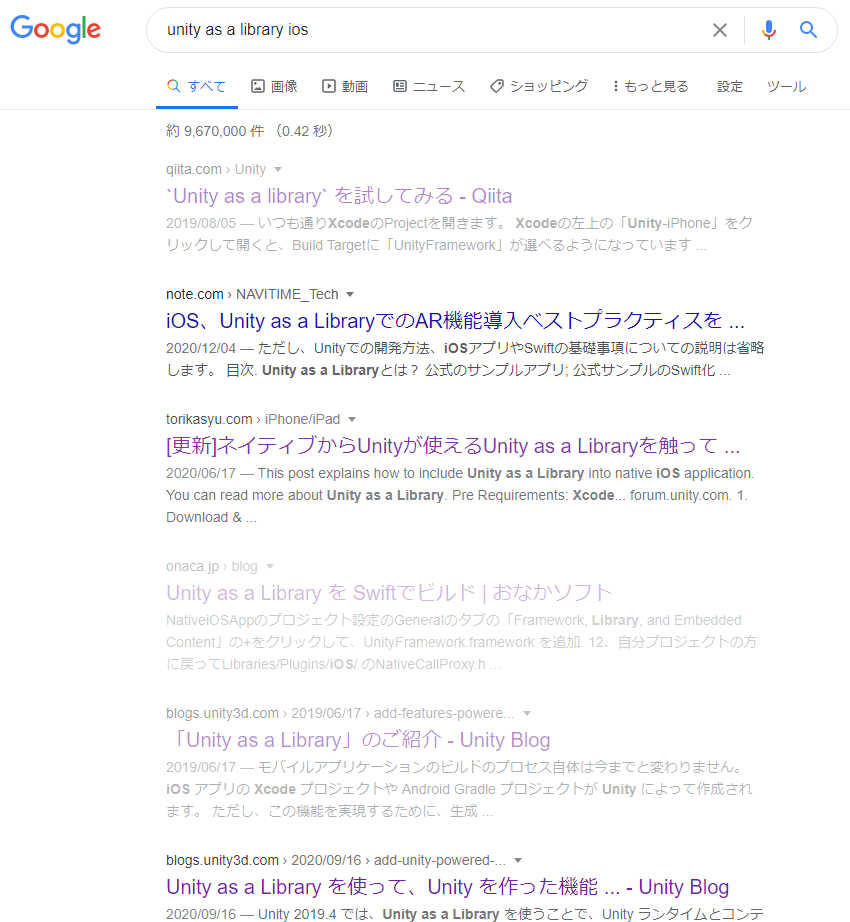
\includegraphics[width=60mm]{images/transparence.png}}
  \end{center}
  \caption{不透明度を変更した視覚化}
  \label{fig:ver-transparence}
\end{figure}

図\ref{fig:ver-transparence}は,各情報ごとに古ければ古いほど不透明度が下がっていくようにしている.

元の検索画面に対して微小な変更のみを加えているため,不自然な点が少ない.また,段階的な変化が認識しやすく時間経過を簡単に見て取れる.

しかし「薄い(不透明度が低い)=古い」という結びつけが弱いため,鮮度を表しているという認識を与えられるか疑問がある.

\subsection{滲む}
\label{subsec:ver-chr-bld}

紙にインクを垂らすとにインクは滲んでいく.そのイメージを参考に,鮮度を視覚化した.

\begin{figure}[htbp]
  \begin{center}
    \fbox{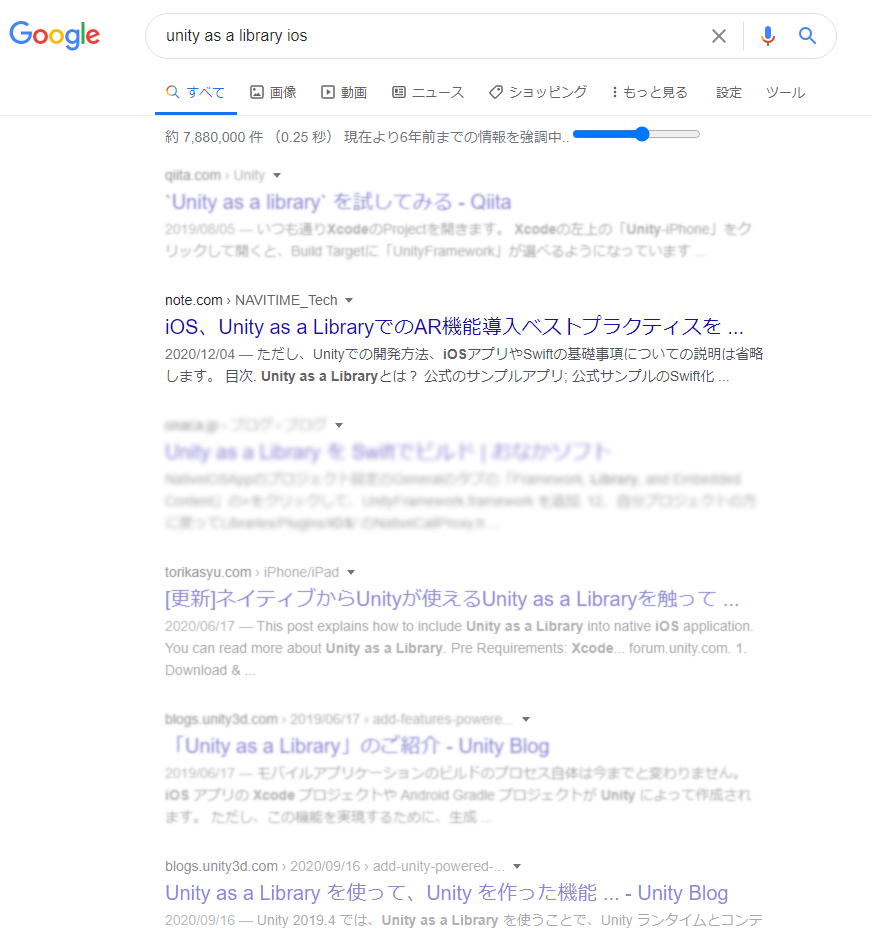
\includegraphics[width=60mm]{images/bleeding.png}}
  \end{center}
  \caption{インクの滲みをイメージした視覚化}
  \label{fig:ver-bleeding}
\end{figure}

図\ref{fig:ver-bleeding}は,\ref{subsec:ver-chr-trp}と同様の基準で文字が滲んでいる.

透明化のように元の背景とよくなじみ,段階的な変化が感じやすい.加えて,古い情報を読ませないという効果も期待できる.

しかし,滲んでいるから古い情報だという結びつけは弱いように思われる.

\subsection{虫食い}
\label{subsec:ver-chr-wh}

古い書物などは紙自体の経年劣化の他にシミなどの虫による欠落が見られる.そういった劣化の仕方を参考に鮮度を視覚化した.

\begin{figure}[htbp]
  \begin{minipage}{0.5\hsize}
    \begin{center}
      \fbox{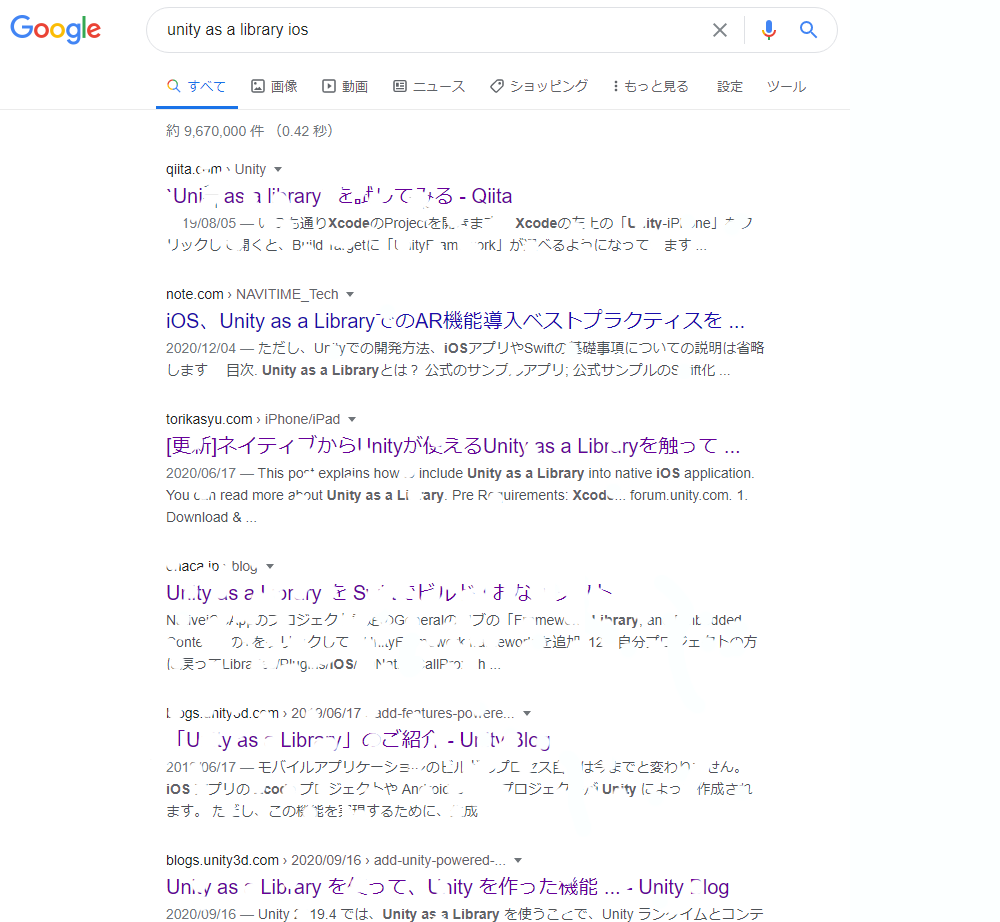
\includegraphics[width=60mm]{images/wormhole1.png}}
    \end{center}
    \caption{虫食いをイメージした視覚化1}
    \label{fig:ver-wormhole1}
  \end{minipage}
  \begin{minipage}{0.5\hsize}
    \begin{center}
      \fbox{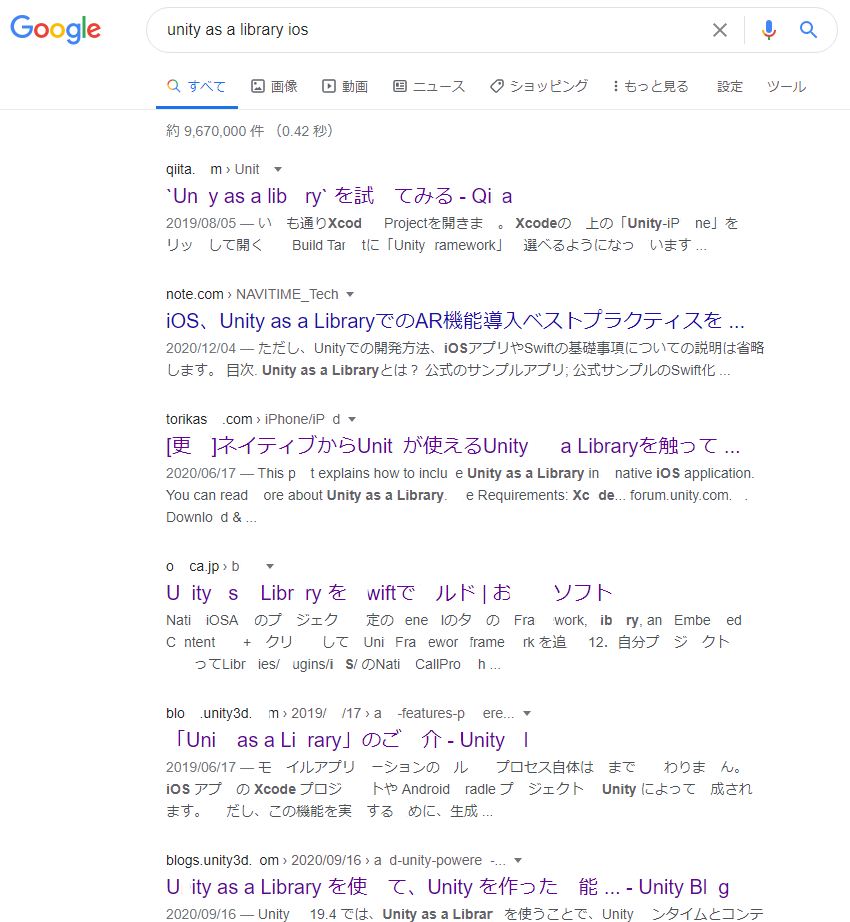
\includegraphics[width=60mm]{images/wormhole2.png}}
    \end{center}
    \caption{虫食いをイメージした視覚化2}
    \label{fig:ver-wormhole2}
  \end{minipage}
\end{figure}

図\ref{fig:ver-wormhole1}は実際に虫に食われた紙をイメージして,古ければより欠損するように視覚化をしている.

図\ref{fig:ver-wormhole2}は文章の虫食いをイメージして,古ければ古いほど多くの文字が欠落するように視覚化をしている.

どちらも情報の鮮度に応じた変化の差を設けるのが難しいが,古い情報を読ませない効果は十分にある.

しかし,ある程度の文字が欠損していても何となく読めてしまう部分があり,\ref{subsec:ver-col-ink}の視覚化と同様,段階的な変化ではなく読めるか読めないかの二分された認識になった.

\section{フォントによる変化}
\label{sec:ver-font}

\subsection{書体}
\label{subsec:ver-fnt-stl}

時代が進むごとに文字の書体も変わってきた\footnote{5分で学ぶフォントの歴史500年|時代背景とタイポグラフィ, https://note.com/smartcamp-design/n/n2740a3b72be9}.

古い情報は古そうだと感じられる書体を,新しい情報は新しそうだと感じられる書体を用いて記述することで情報の鮮度を視覚化した.

\begin{figure}[htbp]
  \begin{center}
    \fbox{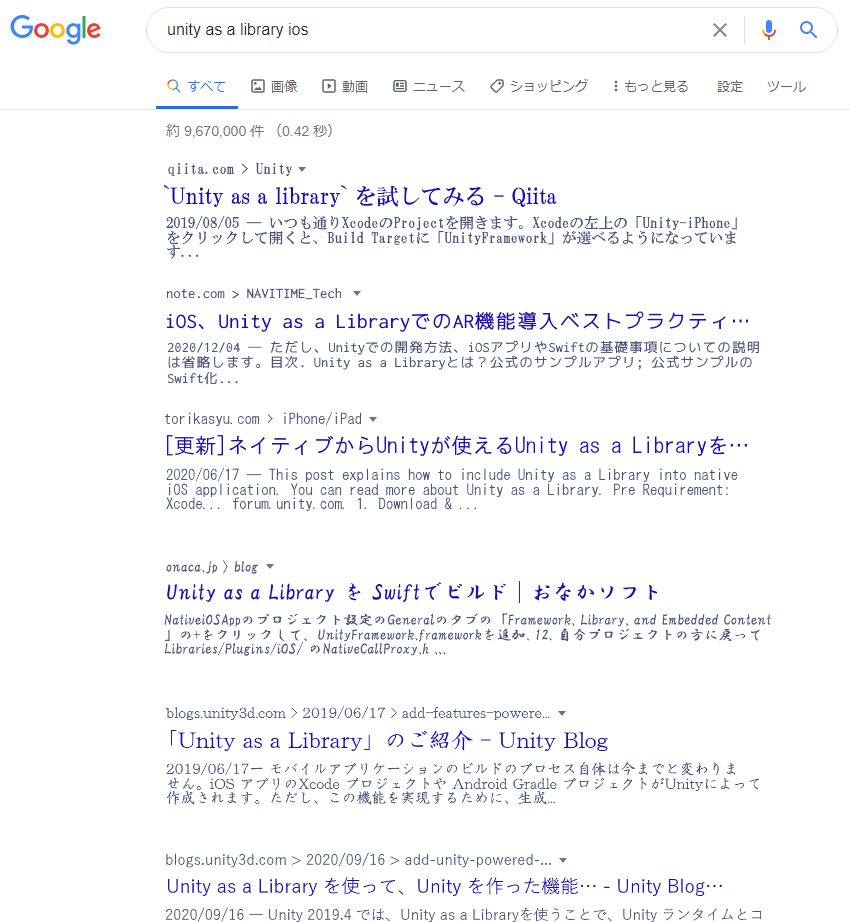
\includegraphics[width=60mm]{images/font-style.png}}
  \end{center}
  \caption{書体の変化による視覚化}
  \label{fig:ver-style}
\end{figure}

図\ref{fig:ver-style}は各情報ごとに Windows に標準で搭載されているフォントを用いて,鮮度を視覚化している.

画像を作成する際に,以下の二つの問題点が見つかった.

\begin{itemize}
  \item フォントの選定が難しい
  \item 人によってフォントに対する印象が違う
\end{itemize}

多数存在するフォントの中から鮮度に合わせたフォントをピックアップするのは難しい.また,フォントを選定した人間の感覚では完璧であっても,第三者が利用する場合に鮮度を認識できない可能性がある.

\subsection{ドット文字}
\label{subsec:ver-fnt-dot}

古い電子機器の画面ではピクセル数の関係からドット文字が使用されていたり,古さを演出するために意図的にドット文字を使うこともある.

そこで粒度の違うドット文字を用いて情報の鮮度を視覚化した.

\begin{figure}[htbp]
  \begin{center}
    \fbox{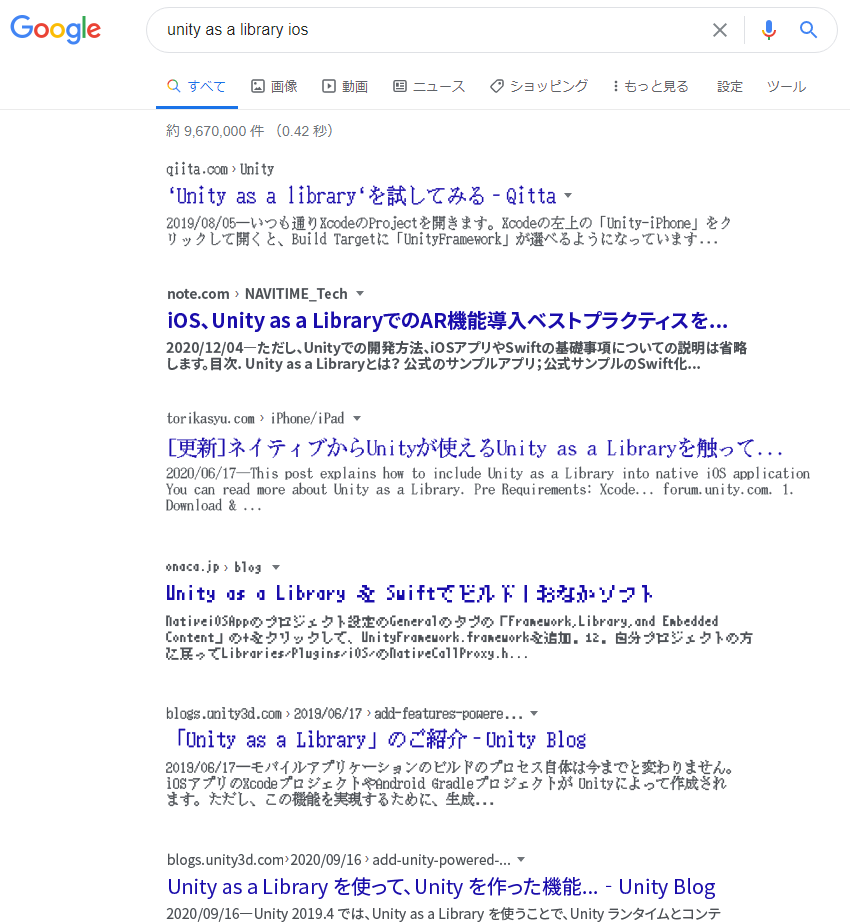
\includegraphics[width=60mm]{images/font-dot.png}}
  \end{center}
  \caption{ドット文字の粒度の変化による視覚化}
  \label{fig:ver-dot}
\end{figure}

図\ref{fig:ver-dot}は,古ければ古いほど粒度の荒いドット文字を使用している.

予測では鮮度の段階ごとの変化を感じやすいと思われたが,古い印象よりも各サイトごとの特色だという印象の方が強かった.

これは各ドット文字がそれぞれ特徴的で,段階的な変化を感じさせなかったためだと推測される.
